%%%%%%%% ICML 2026 SUBMISSION — Learning Beyond Gradients %%%%%%%%%%%%%%%%
% Compile: pdflatex main && bibtex main && pdflatex main && pdflatex main
% Review version (anonymized, line numbers). For camera-ready, switch to
% \usepackage[accepted]{icml2026} and fill in the real author block below.

\documentclass{article}

\usepackage{microtype}
\usepackage{graphicx}
\usepackage{booktabs}
\usepackage{amsmath,amssymb,mathtools,bm}
\usepackage{amsthm}
\usepackage{tikz}
\usetikzlibrary{positioning,arrows.meta}

% hyperref must come before icml2026 (per ICML template)
\usepackage{hyperref}
\newcommand{\theHalgorithm}{\arabic{algorithm}}

\usepackage{icml2026}   % review mode: anonymized + ruler. Use [accepted] for final.

% ---------- theorem setup (numbered within section so Thm 4.2, 5.1, ...) ----
\theoremstyle{plain}
\newtheorem{theorem}{Theorem}[section]
\newtheorem{proposition}[theorem]{Proposition}
\newtheorem{corollary}[theorem]{Corollary}
\newtheorem{lemma}[theorem]{Lemma}
\theoremstyle{definition}
\newtheorem{definition}[theorem]{Definition}
\newtheorem{assumption}[theorem]{Assumption}
\newtheorem{example}[theorem]{Example}
\theoremstyle{remark}
\newtheorem{remark}[theorem]{Remark}

% ---------- macros ----------
\newcommand{\A}{\mathcal{A}}
\newcommand{\Y}{\mathcal{Y}}
\newcommand{\D}{\mathcal{D}}
\newcommand{\M}{\mathcal{M}}
\newcommand{\E}{\mathbb{E}}
\renewcommand{\P}{\mathbb{P}}
\newcommand{\R}{\mathbb{R}}
\newcommand{\N}{\mathbb{N}}
\newcommand{\sel}{\mathrm{sel}}
\newcommand{\len}{\ell}
\newcommand{\Fhat}{\widehat{F}}
\newcommand{\Ftil}{\widetilde{F}}
\newcommand{\eps}{\varepsilon}

\icmltitlerunning{A Unifying Theory of LLM-Guided Artifact Search}

\begin{document}

\twocolumn[
\icmltitle{Learning Beyond Gradients: \\ A Unifying Theory of LLM-Guided Artifact Search}

% Review mode prints "Anonymous Authors". For the camera-ready, replace with
% real names and switch the package option to [accepted].
\icmlsetsymbol{equal}{*}
\begin{icmlauthorlist}
\icmlauthor{Anonymous Authors}{anon}
\end{icmlauthorlist}
\icmlaffiliation{anon}{Anonymous Institution}
\icmlcorrespondingauthor{Anonymous Author}{anon.email@domain.com}

\icmlkeywords{learning beyond gradients, prompt optimization, universal search, language feedback, quality diversity, PAC-Bayes, Goodhart}

\vskip 0.3in
]

\printAffiliationsAndNotice{}

\begin{abstract}
A rapidly growing family of systems improves at tasks without touching model weights: an outer loop proposes edits to a textual or programmatic \emph{artifact}---a prompt, a skill document, an agent harness, a training script---scores each candidate with a noisy evaluator, and keeps what works, with a frozen large language model (LLM) acting as the proposal distribution. Instances include reflective prompt evolution, self-evolving skills and contexts, harness optimization, automated agent design, evolutionary code search, and autonomous ML research. These systems were developed largely independently and are analyzed, when at all, in isolation. We give a single formal model that contains them all, and we prove that its behavior is governed by a small number of quantities: the \emph{prior mass} the proposer places on good artifacts (which controls hitting time, Levin-style), the \emph{information content of feedback} (scalar rewards can be exponentially slower than execution traces), the \emph{noise--gap ratio} of the evaluator (greedy ratchets provably manufacture $\sigma\sqrt{2\ln t}$ of fictitious improvement; $O((\sigma^2/\Delta^2)\log(B/\delta))$ repeated evaluations restore soundness), the \emph{deceptiveness} of the landscape (archive-based selection is exponentially faster than tolerant greedy search), and the \emph{description length} of the artifact (an Occam bound that predicts both context collapse and validation overfitting). We complement the theorems with controlled simulations, and we map each result back to documented behaviors---and documented failures---of deployed systems. The picture that emerges is that ``learning beyond gradients'' is stochastic search over program space with a learned prior and a wide feedback channel: a regime classical theory already speaks to, once the translation is made explicit.
\end{abstract}

\section{Introduction}
\label{sec:intro}

The dominant formal account of machine learning is gradient-based: define a differentiable loss, follow its gradient in weight space. Yet many of the most striking recent gains in LLM-based systems involve no weight updates at all. GEPA evolves prompts by reflecting on execution traces and outperforms the RL algorithm GRPO with up to $35\times$ fewer rollouts \cite{agrawal2025gepa}. Meta-Harness rewrites the scaffolding code around a frozen model and beats hand-built context-management systems \cite{lee2026metaharness}. SkillOpt edits a skill document under held-out acceptance tests and lifts frozen-agent accuracy by double digits \cite{yang2026skillopt}. AlphaEvolve and FunSearch evolve programs against machine-checkable evaluators and produce new mathematics \cite{novikov2025alphaevolve,romeraparedes2024funsearch}. Karpathy's \emph{autoresearch} loop edits a real training codebase overnight and improves a public speedrun benchmark by 11\% \cite{karpathy2026autoresearch}. Heuristic Learning systems patch executable heuristics from replayed failures \cite{weng2026hl}. The Darwin G\"odel Machine and ADAS search over agent designs themselves \cite{zhang2025dgm,hu2025adas}.

Each of these systems was presented with its own vocabulary---reflection, evolution, context engineering, self-improvement---and each paper's analysis, where present, is empirical. This leaves basic questions open. Why are these loops so sample-efficient when classical program search is hopeless? When does a scalar reward suffice and when are traces necessary? Why did the noisy 5-minute evaluations of autoresearch produce celebrated improvements that later failed to replicate? Why do greedy prompt optimizers overfit their validation sets while bounded-edit optimizers generalize? Why do archives and Pareto frontiers keep appearing in independently developed systems?

\textbf{This paper.} We answer these questions in a single model. An \emph{artifact-search system} (Definition~\ref{def:as}) is a tuple $(\A, F, q, \sel, \M)$: a countable space of textual/programmatic artifacts, a noisy evaluator, an LLM proposal kernel conditioned on execution feedback and memory, a selection rule, and an accumulating history. Learning updates the artifact; the model weights never move. Within this model we prove:

\textbf{(1) Prior mass governs hitting time} (\S\ref{sec:prior}). The expected number of proposals before an $\eps$-good artifact appears is exactly the inverse of the probability mass the proposer assigns to the good set, and adaptive trace-conditioning enters as a multiplicative boost (Theorem~\ref{thm:hitting}); a matching lower bound holds (Proposition~\ref{prop:hitlower}). This is an adaptive form of Levin's universal-search bound \cite{levin1973universal} and formalizes the folk claim that pretraining is what makes text-space search affordable: \emph{sample efficiency is prior mass}.

\textbf{(2) Feedback is a channel, and its information content separates learning rates} (\S\ref{sec:feedback}). Identification with binary success feedback requires $\Omega(2^L)$ queries on $L$-bit artifact classes, while structured feedback that names the first failure needs at most $L$ (Theorem~\ref{thm:separation}); a transcript-counting bound interpolates between these regimes (Theorem~\ref{thm:fano}). This is a self-contained, worst-case companion to the eluder-dimension theory of learning from language feedback \cite{xu2025llf}, and it formalizes why trace-reading optimizers beat scalar-reward RL at small budgets.

\textbf{(3) Noise makes greedy ratchets unsound, quantifiably} (\S\ref{sec:selection}). A single-evaluation ratchet fed pure-noise edits reports $\sigma\sqrt{2\ln t}$ of improvement after $t$ candidates while making $\ln t$ false accepts---both with matching simulations---whereas $N = O((\sigma^2/\Delta^2)\log(B/\delta))$ repeated evaluations per decision certify a whole $B$-step run (Theorem~\ref{thm:ratchet}, Corollary~\ref{cor:budget}). The autoresearch episode is this theorem executed in public.

\textbf{(4) Deception separates greedy from archive selection} (\S\ref{sec:selection}). On an explicit deceptive landscape, strict greedy search never reaches the optimum, $\eps$-tolerant greedy needs $\exp(\Omega(k))$ steps to cross a width-$k$ valley, and an archive-based novelty rule arrives in $O(k^2)$ (Theorem~\ref{thm:deception}). This is the formal content of the quality-diversity design choices---Pareto frontiers, agent archives, lineages---recurring across GEPA, ADAS, and the DGM.

\textbf{(5) The artifact is a compressed posterior, and description length controls generalization} (\S\ref{sec:compression}). An Occam/PAC-Bayes bound for artifact selection yields a U-shaped risk in artifact length that simultaneously explains \emph{context collapse} (too short) and validation overfitting (too long), and justifies bounded-edit acceptance discipline (Theorem~\ref{thm:occam}, Corollary~\ref{cor:ushape}).

\textbf{(6) Proxy gaps bound the whole enterprise} (\S\ref{sec:limits}). Measured progress transfers to true progress up to twice the evaluator's bias sup-norm; selection pressure harvests bias at rate $\sigma_b\sqrt{2\ln m}$ (the optimizer's curse); and if the loop can modify its own evaluator, no transfer guarantee survives (Proposition~\ref{prop:goodhart}). This locates the Goodhart failure modes documented across deployed systems and gives the integrity condition that separates them from sound self-improvement.

Sections~\ref{sec:experiments}--\ref{sec:related} provide simulations and situate the framework; proofs are in the appendices. Our aim is the one articulated for the reward hypothesis by \citet{bowling2023settling}: not to introduce a new algorithm, but to settle what a fast-moving empirical literature is, mathematically, so that its successes and failures become predictions rather than surprises.

\section{One Loop, Many Names: the Formal Model}
\label{sec:model}

\begin{figure}[t]
\centering
\resizebox{\columnwidth}{!}{%
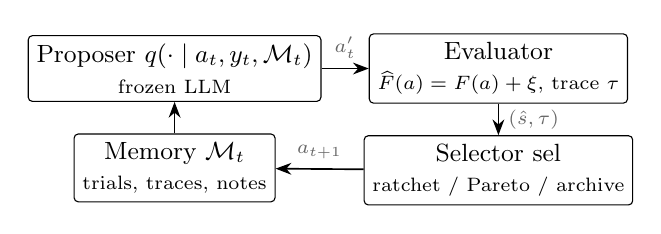
\begin{tikzpicture}[
  node distance=4mm and 6mm,
  box/.style={draw, rounded corners=1.5pt, align=center, inner sep=3pt, font=\small},
  lab/.style={font=\scriptsize\itshape, text=black!60},
  arr/.style={-{Stealth[length=2mm]}, semithick}
]
\node[box] (prop) {Proposer $q(\cdot \mid a_t, y_t, \M_t)$\\ \scriptsize frozen LLM};
\node[box, right=of prop] (eval) {Evaluator\\ \scriptsize $\Fhat(a) = F(a) + \xi$, trace $\tau$};
\node[box, below=of eval] (sel) {Selector $\sel$\\ \scriptsize ratchet / Pareto / archive};
\node[box, below=of prop] (mem) {Memory $\M_t$\\ \scriptsize trials, traces, notes};
\draw[arr] (prop) -- node[lab, above] {$a'_{t}$} (eval);
\draw[arr] (eval) -- node[lab, right] {$(\hat{s}, \tau)$} (sel);
\draw[arr] (sel) -- node[lab, above] {$a_{t+1}$} (mem);
\draw[arr] (mem) -- node[lab, right] {} (prop);
\end{tikzpicture}%
}
\caption{The artifact-search loop. Weights are frozen everywhere; learning is the trajectory $a_0, a_1, \dots$ through artifact space. Systems differ only in $\A$, the feedback alphabet, and $\sel$ (Table~\ref{tab:systems}).}
\label{fig:loop}
\end{figure}

\begin{definition}[Artifact-search system]
\label{def:as}
An \emph{artifact-search system} is a tuple $\mathcal{S} = (\A, F, q, \sel, \M)$ where
(i) $\A$ is a countable set of \emph{artifacts} (finite strings: prompts, skill documents, programs, harness code);
(ii) $F : \A \to [0,1]$ is the \emph{true score}, $F(a) = \E_{z \sim \D}[s(a, z)]$ for a task distribution $\D$ and bounded per-instance score $s$, accessed only through noisy evaluations $\Fhat$ and through \emph{feedback} $y \in \Y$ (a scalar, a trace, an error message, a video);
(iii) $q(\cdot \mid a, y, \M)$ is the \emph{proposer}, a fixed conditional distribution over $\A$ realized by a frozen LLM prompted with the current artifact, feedback, and memory;
(iv) $\sel$ is a \emph{selection rule} mapping evaluated candidates to the retained state (a single incumbent, a Pareto set, an archive, a lineage);
(v) $\M_t$ is accumulated history.
A \emph{run} is the induced stochastic process $a_0, a_1, \ldots$; for $\eps \ge 0$ the \emph{good set} is $G_\eps = \{a : F(a) \ge \sup_{a'} F(a') - \eps\}$, and the \emph{hitting time} is $T = \min\{t : a_t \in G_\eps\}$.
\end{definition}

The definition is deliberately minimal, and that is the point: the systems in Table~\ref{tab:systems} differ in engineering but not in type. Learning happens \emph{in artifact space}; the gradient-trained model appears only as the fixed kernel $q$. Three structural facts drive everything that follows. First, $\A$ is discrete and enormous, so all guarantees must come from where $q$ puts its mass (\S\ref{sec:prior}). Second, the loop's only contact with the task is the feedback channel $\Y$, so its informativeness rate-limits learning (\S\ref{sec:feedback}). Third, $\Fhat$ is noisy and expensive, so selection is statistics, not bookkeeping (\S\ref{sec:selection}).

\begin{table}[t]
\caption{Deployed systems as artifact-search systems. (Feedback abbreviations: sc.\ = scalar score; tr.\ = execution trace.)}
\label{tab:systems}
\vskip 0.1in
\centering
\small
\setlength{\tabcolsep}{3.2pt}
\resizebox{\columnwidth}{!}{%
\begin{tabular}{@{}llll@{}}
\toprule
System & Artifact $\A$ & Feedback $\Y$ & $\sel$ \\
\midrule
GEPA & prompts & sc.\ + tr. & instance-Pareto \\
SkillOpt & skill doc & sc.\ + tr. & gated ratchet \\
ACE & context/playbook & tr. & curated incumbent \\
Meta-Harness & harness code & sc.\ + raw history & ratchet \\
autoresearch & training code & sc.\ (noisy) & greedy ratchet \\
Heuristic Learning & heuristic code & tr.\ (logs, video) & gated ratchet \\
ADAS / DGM & agent programs & sc.\ + tr. & archive / lineage \\
FunSearch / AlphaEvolve & programs & sc.\ (verified) & island archive \\
OPRO / APE / PromptBreeder & prompts & sc. & population \\
Voyager & skill library & tr. & additive library \\
\bottomrule
\end{tabular}%
}
\vskip -0.1in
\end{table}

\paragraph{Where the inner magic lives.}
Our results treat $q$ as a black-box measure. The reason a frozen LLM is a \emph{useful} measure is the subject of the in-context-learning literature: conditioning behaves like implicit Bayesian inference \cite{xie2022explanation, akyurek2023what}, and trained transformers can emulate learning algorithms in context \cite{vonoswald2023transformers, garg2022what}. We import this as licence for the modeling assumption that feedback conditioning \emph{increases} $q(G_\eps)$---Assumption~\ref{ass:boost} below---and otherwise remain agnostic about mechanism.

\paragraph{Relation to classical objects.}
With $q$ fixed and $\Y$ trivial, Definition~\ref{def:as} is randomized program search, and Levin's universal search \cite{levin1973universal, solomonoff1964formal} with its modern descendants \cite{schmidhuber2004oops, schmidhuber1997shifting, hutter2005universal, achille2025universal} applies verbatim. With $\A$ a population and $\sel$ an archive, it is quality-diversity evolution \cite{lehman2011abandoning, mouret2015illuminating}. With $\sel$ statistical and $\Fhat$ noisy, it is best-arm identification \cite{maron1994hoeffding, evendar2006action, karnin2013almost, li2017hyperband}. The contribution of this paper is to make the translations exact and extract the quantitative consequences for the LLM-era instantiations.

\section{Resource I: Prior Mass}
\label{sec:prior}

No search rule can beat uniform enumeration on average over all problems \cite{wolpert1997no}; concretely, Theorem~\ref{thm:separation}(i) below implies that for a uniformly placed target in a space of size $|\A|$, \emph{every} algorithm has expected hitting time $(|\A|+1)/2$. Whatever makes artifact search tractable must therefore be alignment between the proposer and the problem. The following theorem says this alignment is measured by one number.

\begin{assumption}[Trace boost]
\label{ass:boost}
There exist $\gamma_t \ge 0$ such that, almost surely over histories, the conditioned proposer satisfies $q(G_\eps \mid a_t, y_t, \M_t) \ge \gamma_t\, q_0(G_\eps)$, where $q_0$ is the unconditioned (cold) proposal distribution.
\end{assumption}

\begin{theorem}[Hitting time = inverse prior mass]
\label{thm:hitting}
Let proposals $a'_1, a'_2, \ldots$ be drawn from the system's proposer and let $T$ be the first time $a'_t \in G_\eps$.
\begin{enumerate}\itemsep1pt
\item[(i)] If proposals are i.i.d.\ from $q$ with $p \coloneqq q(G_\eps) > 0$, then $\E[T] = 1/p$, and $T \le \ln(1/\delta)/p$ with probability $\ge 1-\delta$.
\item[(ii)] If each proposal costs compute $c(a)$ with $\bar{c} = \E_{a \sim q}[c(a)] < \infty$, the expected total compute is $\E\big[\sum_{t \le T} c(a'_t)\big] = \bar{c}/p$.
\item[(iii)] Under Assumption~\ref{ass:boost} with $\gamma_t \ge \gamma > 0$ for all $t$, $\E[T] \le 1/(\gamma\, q_0(G_\eps))$, and more generally $\E[T] \le t_0 + 1/(\gamma\, q_0(G_\eps))$ if the bound holds only for $t \ge t_0$.
\end{enumerate}
\end{theorem}

\begin{proposition}[Lower bound]
\label{prop:hitlower}
If instead $q(G_\eps \mid \cdot) \le \bar{q}$ almost surely at every step, then $\E[T] \ge 1/(2\bar{q}) - 1$.
\end{proposition}

Proofs are in Appendix~\ref{app:prior}; (ii) is Wald's identity \cite{wald1944cumulative}, and the pair (i)+(iii) is an adaptive analogue of Levin's bound, in which search cost is inverse prior mass weighted by per-program time \cite{levin1973universal}. Three readings matter for practice.

\emph{Pretraining buys $q_0(G_\eps)$.} The cold prior mass a frontier model puts on ``useful edits to this artifact'' is the quantity that moved between 2017-era neural program search \cite{zoph2017nas} and FunSearch: the search algorithm barely changed; the prior did. This is also the formal content of viewing agents as devices that convert pretraining into search-time speedup \cite{achille2025universal}.

\emph{Traces buy $\gamma_t$.} Feedback conditioning multiplies, rather than adds to, the cold mass: a proposer that reads a stack trace and localizes the fault concentrates $q$ on the small set of edits consistent with it. Section~\ref{sec:feedback} bounds how large this multiplier can be in terms of the information carried by $y$. The same mechanism run backward is a warning: misleading feedback ($\gamma < 1$) provably \emph{slows} search below cold sampling (Proposition~\ref{prop:hitlower}), a regime documented when traces are uninformative for the failure mode at hand, e.g.\ sparse-reward exploration domains \cite{weng2026hl}.

\emph{Reuse compounds the prior.} Adding solved-task artifacts to $\M$ (skill libraries in Voyager, candidate pools in GEPA, lineages in DGM) re-weights $q_0$ for subsequent problems---the mechanism of incremental bias shift formalized for program search by \citet{schmidhuber1997shifting, schmidhuber2004oops}.

\section{Resource II: Feedback Information}
\label{sec:feedback}

Fix the prior; what does richer feedback buy? We model one round as: the learner proposes $a \in \A$, and a feedback oracle returns $y = \phi(a, a^*) \in \Y$, where $a^*$ is an unknown target artifact (the ``right'' prompt, patch, or program) and $\phi$ is the feedback protocol. Identification of $a^*$ is the cleanest possible stand-in for ``learning the task''; richer settings reduce to it locally.

\begin{theorem}[Transcript bound]
\label{thm:fano}
Let $\A^* \subseteq \A$ with $|\A^*| = 2^L$ and let $a^*$ be uniform on $\A^*$. Any (possibly randomized) algorithm that identifies $a^*$ within $T$ rounds with probability $\ge 1/2$, using feedback alphabet $\Y$ with $|\Y| \ge 2$, satisfies
\[
T \;\ge\; \frac{L - \log_2 6}{\log_2 |\Y|}.
\]
\end{theorem}

\begin{theorem}[Exponential separation]
\label{thm:separation}
Let $\A^* = \{0,1\}^L$ and $a^*$ uniform.
\begin{enumerate}\itemsep1pt
\item[(i)] \textbf{Scalar success reward} ($\phi = \mathbf{1}\{a = a^*\}$): every algorithm has $\E[T] \ge (2^L + 1)/2$.
\item[(ii)] \textbf{First-error feedback} ($\phi$ = index of the first coordinate where $a$ disagrees with $a^*$): a deterministic algorithm identifies $a^*$ in at most $L$ rounds.
\item[(iii)] \textbf{Distance feedback} ($\phi$ = Hamming distance): $L + 1$ rounds suffice.
\end{enumerate}
\end{theorem}

The gap between (i) and (ii) is $2^L$ vs.\ $L$: \emph{exponential}, and not an artifact of alphabet size---first-error feedback uses an alphabet of size $L{+}1$, only logarithmically wider as measured by Theorem~\ref{thm:fano}, yet realizes exponentially more \emph{usable} information because each response certifies a prefix and names a fault. This is precisely the structure of a stack trace, a failed unit test with its name, or a judge critique that says \emph{where} the rollout went wrong. The general theory of when language feedback admits such speedups is developed by \citet{xu2025llf} via the transfer eluder dimension, with benchmark instantiations in \citet{cheng2023llfbench}; Theorem~\ref{thm:separation} is the minimal worst-case example one can keep in one's head, in the lineage of Shannon's dictum that information is what reduces uncertainty \cite{shannon1948mathematical, cover2006elements}.

Reading the empirical record through this lens: GEPA's advantage over GRPO at matched rollout budgets \cite{agrawal2025gepa} is the prediction of (i)-vs-(ii) for systems that read traces versus systems that collapse rollouts to scalars; the same comparison recurs as TextGrad's textual gradients \cite{yuksekgonul2024textgrad}, Trace's execution-graph feedback \cite{cheng2024trace}, Reflexion's verbal self-feedback \cite{shinn2023reflexion}, and Meta-Harness's insistence on exposing \emph{raw} histories rather than summaries \cite{lee2026metaharness}. Conversely, scalar-only loops are not doomed---they are slow by exactly the measure of Theorem~\ref{thm:fano}, which is why they appear where evaluation is verified and cheap (FunSearch's island model makes millions of scalar-scored calls \cite{romeraparedes2024funsearch}).

\section{Selection: Noise and Deception}
\label{sec:selection}

The selector sees neither $F$ nor $a^*$; it sees $\Fhat = F + \xi$ under an evaluation budget. Two independent hazards arise: \emph{statistical} (noise creates fictitious progress) and \emph{geometric} (real progress requires descending). Both have sharp, elementary theory; both have been rediscovered empirically at some cost.

\subsection{The Ratchet Illusion}

Model a worst case that is also the common case at the frontier of a tuned system: a stream of \emph{null edits}, each with true gain $0$, evaluated once with $\sigma$-subgaussian noise. The greedy single-evaluation ratchet (accept iff the measured score beats the incumbent's measured score) is exactly the rule of autoresearch \cite{karpathy2026autoresearch} and of naive prompt hill-climbing.

\begin{theorem}[Ratchet illusion]
\label{thm:ratchet}
Let $\hat{s}_1, \dots, \hat{s}_t$ be the measured scores of $t$ null edits, i.i.d.\ $\sigma$-subgaussian, and let $m_t = \max_{i \le t} \hat{s}_i$ be the reported best.
\begin{enumerate}\itemsep1pt
\item[(i)] $\E[m_t] \le \sigma\sqrt{2 \ln t}$, and for Gaussian noise $\E[m_t] \ge (1 - o(1))\,\sigma\sqrt{2\ln t}$: the reported improvement diverges although every artifact is worthless.
\item[(ii)] The expected number of accepted edits is $H_t = \sum_{i \le t} 1/i = \ln t + O(1)$, independent of $\sigma$.
\end{enumerate}
\end{theorem}

\begin{proposition}[Cost of a sound decision]
\label{prop:repeats}
To distinguish a true gain $\Delta$ from a null edit with both error probabilities $\le \delta$, it suffices to average $N \ge (16\sigma^2/\Delta^2)\ln(1/\delta)$ fresh evaluations per side and accept iff the measured gain exceeds $\Delta/2$; conversely, any rule with both errors $\le \delta$ requires $N \ge (2\sigma^2/\Delta^2)\ln(1/(2\delta))$.
\end{proposition}

\begin{corollary}[Certifying a whole run]
\label{cor:budget}
A $B$-decision loop that applies Proposition~\ref{prop:repeats} with $\delta' = \delta/B$ makes no false accept during the entire run with probability $\ge 1 - \delta$, at per-decision cost $N = O\!\big((\sigma^2/\Delta^2)\log(B/\delta)\big)$: soundness costs only a $\log B$ factor.
\end{corollary}

Theorem~\ref{thm:ratchet} is extreme-value theory \cite{boucheron2013concentration} plus the classical record-counting identity; Proposition~\ref{prop:repeats} is a two-point testing bound \cite{tsybakov2009introduction, hoeffding1963probability}. The practical content is blunt. A loop making $B = 2000$ single-evaluation decisions at $\sigma = \Delta$ will report meaningful-looking progress on pure noise ($\approx 3.9\sigma$, Figure~\ref{fig:ratchet}a) and accept $\approx 7.6$ null edits; the \emph{same} loop with $N = 85$ repeats per decision is sound for the whole run at 5\% (Figure~\ref{fig:ratchet}b). The 11\% autoresearch speedup that survived independent re-evaluation, and the widely circulated ``53\% speedup'' that did not, differ by exactly this discipline; racing and successive-halving methods exist to spend those $N$ evaluations adaptively \cite{maron1994hoeffding, karnin2013almost, li2017hyperband}, and instance-aggregation designs in benchmark construction serve the same theorem \cite{anonymous2026shopgym}.

\subsection{Deception: when descending is necessary}

Noise aside, greedy selection fails on landscapes where the path to the optimum passes through worse artifacts---\emph{deception} in the evolutionary-computation sense \cite{lehman2011abandoning, stanley2015greatness}. We exhibit the cleanest separation we know of.

\begin{theorem}[Deception separation]
\label{thm:deception}
Let $\A = \{0, 1, \dots, 2k\}$ be a chain with local proposals (move to a uniformly random neighbor), $f(i) = k - i$ on $[0, k]$ and $f(i) = i - k$ on $[k, 2k]$, so the unique global optimum is $2k$ and the slope on $[0,k]$ points away from it. Start at $0$.
\begin{enumerate}\itemsep1pt
\item[(i)] \textbf{Strict greedy} (accept only improvements) never reaches $2k$: it halts at $0$ with hitting time $\infty$.
\item[(ii)] \textbf{Tolerant greedy} (accept worsening moves with probability $\eps \in (0,1)$) has $\E[T] \ge 2\,\eps^{-k}$.
\item[(iii)] \textbf{Archive search} (keep all visited artifacts; expand a uniformly random archive member by a random neighbor; ignore $f$ entirely until the end) has $\E[T] \le 4k(2k+1) = O(k^2)$.
\end{enumerate}
\end{theorem}

The proof of (ii) is a birth--death drift computation; (iii) is a frontier argument (Appendix~\ref{app:deception}). The theorem licenses a unification that practitioners reached by convergent evolution: GEPA's per-instance Pareto frontier keeps candidates that are best at \emph{something} even when worse on average \cite{agrawal2025gepa}; ADAS retains an archive of all discovered agents \cite{hu2025adas}; the DGM maintains an expanding lineage and explicitly credits open-endedness \cite{zhang2025dgm}; FunSearch's islands are archives with migration \cite{romeraparedes2024funsearch}. All are mechanisms for buying polynomial valley-crossing at the price of evaluating diverse, currently-worse artifacts---MAP-Elites logic \cite{mouret2015illuminating} transplanted to text space. The theorem also delimits the claim: on deception-free landscapes greedy is optimal among these rules, which is why bounded, well-gated ratchets (SkillOpt, Heuristic Learning) thrive on tasks where each failure names its own fix.

\section{Generalization: the Artifact as Compression}
\label{sec:compression}

What is the evolved artifact, statistically? It is chosen \emph{because} it scored well on $n$ validation instances; its value is its score on fresh ones. Since artifacts are strings, the right uniform-convergence currency is description length, in the MDL tradition \cite{rissanen1978modeling} and its PAC-Bayes form \cite{mcallester1999pac}.

\begin{theorem}[Occam bound for artifact selection]
\label{thm:occam}
Fix a prefix-free code with lengths $\len(a)$ (bits) on $\A$, let $\Fhat_n(a)$ be the mean score on $n$ i.i.d.\ validation instances, and let $\delta \in (0,1)$. With probability $\ge 1 - \delta$, simultaneously for \emph{all} $a \in \A$---hence for the selected $\hat{a}$, no matter how adaptively chosen---
\[
\big|F(a) - \Fhat_n(a)\big| \;\le\; \sqrt{\frac{\len(a) \ln 2 + \ln(2/\delta)}{2n}}.
\]
\end{theorem}

\begin{corollary}[The U-shape: collapse vs.\ bloat]
\label{cor:ushape}
Let $A(L) = \sup_a F(a) - \max_{\len(a) \le L} F(a)$ be the approximation error of length-$L$ artifacts and let $\hat{a}_L$ maximize $\Fhat_n$ over $\{\len(a) \le L\}$. Then with probability $\ge 1-\delta$,
\[
\sup_a F(a) - F(\hat{a}_L) \;\le\; A(L) + 2\sqrt{\frac{L \ln 2 + \ln(2/\delta)}{2n}} .
\]
\end{corollary}

The two terms move in opposite directions in $L$, and the corollary is a quantitative statement of the two documented failure modes of context evolution \cite{zhang2025ace}: \emph{context collapse} is operating at $L$ below the knee of $A(L)$---the artifact is too short to encode the task statistic it is supposed to carry---while \emph{validation overfitting} is letting $L$ grow with $n$ fixed, the regime in which GEPA-style optimizers are observed to degrade on held-out instances. It also derives, rather than assumes, two disciplines that the strongest gated systems adopted empirically: SkillOpt's bounded add/delete/replace edits control the growth of $\len(a)$ per accepted step \cite{yang2026skillopt}, and Heuristic Learning's instruction to ``absorb feedback \emph{and} compress history'' \cite{weng2026hl} is explicit description-length management; memory-curation systems live in the same trade-off \cite{packer2023memgpt, suzgun2025cheatsheet}. The bound's $\sqrt{\len/n}$ scaling makes a falsifiable prediction: validation set size must grow linearly in artifact bits to keep the certified gap constant.

\section{Limits: Proxy Gaps and Self-Reference}
\label{sec:limits}

Every guarantee so far conditions on the evaluator measuring what we mean. Let $\Ftil = F + b$ be the proxy actually optimized, with bias $b$ (judge error, reward misspecification, test-set leakage).

\begin{proposition}[Goodhart transfer and its failure]
\label{prop:goodhart}
\begin{enumerate}\itemsep1pt
\item[(i)] \textbf{Bounded bias transfers.} If $|b(a)| \le \alpha$ on all reachable artifacts and a run certifies measured progress $\Ftil(a_T) - \Ftil(a_0) \ge g$, then $F(a_T) - F(a_0) \ge g - 2\alpha$.
\item[(ii)] \textbf{Selection harvests bias.} If $\hat{a}$ maximizes $\Ftil$ over $m$ candidates whose biases are independent $\sigma_b$-subgaussian, the harvested bias satisfies $\E[b(\hat{a})] \le \sigma_b \sqrt{2 \ln m}$, and this rate is attained for Gaussian bias on otherwise-equal candidates.
\item[(iii)] \textbf{Evaluator integrity is necessary.} If the loop can modify the map $a \mapsto b(a)$ along reachable paths (an editable evaluator), there exist systems with $\Ftil(a_t) \uparrow \infty$ and $F(a_t) \downarrow -\infty$: no transfer guarantee holds.
\end{enumerate}
\end{proposition}

Part (ii) is the optimizer's curse expressed for artifact search: optimization pressure converts evaluator variance into systematic overestimate at a $\sqrt{2\ln m}$ rate---\emph{regressional} Goodhart in the taxonomy of \citet{manheim2018categorizing}---which compounds the noise effects of Theorem~\ref{thm:ratchet}. Part (iii) is the \emph{adversarial} corner: its hypothesis sounds exotic until one recalls documented instances---agents hallucinating tool logs to satisfy checks in the DGM \cite{zhang2025dgm}, evolved reward functions exploiting simulator physics \cite{ma2024eureka}, metric gaming in autonomous-research loops---all special cases of reward hacking \cite{amodei2016concrete}. The constructive reading: freeze the evaluator, hold it out from the proposer's edit scope, and re-estimate bias on fresh data, and (i)+(ii) bound the damage; let the loop touch it and the guarantee is not weakened but \emph{void}. The self-referential limit---improvers improving improvers \cite{schmidhuber2003godel, zelikman2024stop, fernando2023promptbreeder}---inherits exactly this condition, and we record in Appendix~\ref{app:open} the open problem of rates: how fast must evaluator gap shrink, relative to growing optimization pressure, for $\mathrm{improve}(\mathrm{improver})$ to converge \cite{yampolskiy2015seed, chalmers2010singularity}?

\section{Numerical Illustrations}
\label{sec:experiments}

We validate the three quantitative theorems in controlled simulation; code is in the supplement and all figures regenerate in under a minute on a laptop. These are illustrations of exact statements, not benchmark claims.

\begin{figure*}[t]
\centering

\includegraphics[width=\textwidth]{figures/fig_ratchet.pdf}
\caption{The ratchet illusion (Theorem~\ref{thm:ratchet}, Corollary~\ref{cor:budget}). Null edits, $\sigma = 1$, 400 runs. \textbf{(a)} Reported best score of a single-evaluation greedy ratchet (median, 10--90\% band) against the $\sigma\sqrt{2\ln t}$ law; the true value of every artifact is $0$. \textbf{(b)} Accepted null edits match $H_t \approx \ln t$; gating each decision with $N = 85$ repeats (the Corollary~\ref{cor:budget} prescription for $B = 2000$, $\delta = 0.05$, $\Delta = \sigma$) eliminates false accepts entirely.}
\label{fig:ratchet}
\end{figure*}

\begin{figure}[t]
\centering

\includegraphics[width=\columnwidth]{figures/fig_feedback.pdf}
\caption{Feedback separation (Theorems~\ref{thm:fano}--\ref{thm:separation}). Mean queries to identify an $L$-bit target under three feedback protocols (60 runs; markers) against the exact laws (dashed). The gap between scalar success reward and first-error feedback is exponential.}
\label{fig:feedback}
\end{figure}

\begin{figure}[t]
\centering

\includegraphics[width=\columnwidth]{figures/fig_deception.pdf}
\caption{Deception separation (Theorem~\ref{thm:deception}). Steps to cross a deceptive valley of half-width $k$: tolerant greedy ($\eps = 0.3$; exact expectation and simulation) grows exponentially; archive search stays under the $4k(2k+1)$ bound. Strict greedy never arrives (not plottable).}
\label{fig:deception}
\end{figure}

Figure~\ref{fig:ratchet} shows the single-evaluation ratchet manufacturing a $\approx 3.9\sigma$ ``improvement'' from 2000 worthless edits, hugging the $\sigma\sqrt{2\ln t}$ curve, with false accepts tracking $H_t$; the $N{=}85$ gate of Corollary~\ref{cor:budget} flattens both. Figure~\ref{fig:feedback} realizes the exponential-vs-linear separation of Theorem~\ref{thm:separation} numerically. Figure~\ref{fig:deception} shows tolerant greedy's exponential wall against the archive's quadratic crossing, including the exact birth--death expectation. Appendix~\ref{app:exp} contains parameters and additional runs.

\section{Related Work}
\label{sec:related}

\textbf{Empirical beyond-gradient systems.} Prompt optimization spans APE, OPRO, EvoPrompt-style evolution, and program-level compilers \cite{zhou2023ape, yang2024opro, fernando2023promptbreeder, khattab2024dspy, opsahlong2024mipro}, culminating in trace-reflective methods \cite{agrawal2025gepa, yuksekgonul2024textgrad, cheng2024trace}. Context and memory evolution includes ACE, MemGPT, and test-time memory \cite{zhang2025ace, packer2023memgpt, suzgun2025cheatsheet}; skills and heuristics, \cite{yang2026skillopt, weng2026hl, wang2023voyager}; agent/harness search, \cite{hu2025adas, zhang2025dgm, lee2026metaharness}; code and discovery loops, \cite{romeraparedes2024funsearch, novikov2025alphaevolve, karpathy2026autoresearch}; self-referential variants, \cite{zelikman2024stop}. We add no system; we add the common load-bearing mathematics.

\textbf{Theory.} Our prior-mass results adapt universal search \cite{levin1973universal, schmidhuber2004oops, hutter2005universal} and its recent agentic reading \cite{achille2025universal}. The feedback results are worst-case companions to learning from language feedback via transfer eluder dimension \cite{xu2025llf, cheng2023llfbench}, against the scalar-sufficiency position of \citet{silver2021reward}: our account is quantitative rather than oppositional---scalars suffice in the limit, traces change the \emph{rate}, and at frontier evaluation costs the rate is the object of interest. Selection-under-noise imports best-arm identification \cite{evendar2006action, karnin2013almost, li2017hyperband}; deception imports quality-diversity theory \cite{lehman2011abandoning, mouret2015illuminating} and runtime analysis of evolutionary algorithms \cite{droste2002analysis}; generalization imports MDL/PAC-Bayes \cite{rissanen1978modeling, mcallester1999pac}; limits import No Free Lunch \cite{wolpert1997no} and Goodhart taxonomies \cite{manheim2018categorizing, amodei2016concrete}. Methodologically we follow the settle-the-question genre of \citet{bowling2023settling} and \citet{richens2025general}: take a practice the field already trusts and exhibit the theorem it was implicitly assuming.

\section{Discussion and Conclusion}
\label{sec:discussion}

\textbf{One loop, five dials.} The model of Definition~\ref{def:as} reduces a crowded design space to five measurable quantities: cold prior mass $q_0(G_\eps)$, trace boost $\gamma$, feedback information per rollout, noise--gap ratio $\sigma^2/\Delta^2$, and artifact description length $\len(a)$---plus one integrity condition on the evaluator. Each theorem turns a current engineering slogan into a falsifiable scaling claim: hitting time should scale inversely with measured prior mass (testable by ablating proposer quality); scalar-vs-trace gaps should scale with the feedback's usable bits (testable by degrading traces); required repeats should scale as $\sigma^2/\Delta^2 \cdot \log B$ (testable in any ratchet); certified generalization gaps should scale as $\sqrt{\len(a)/n}$ (testable across artifact sizes).

\textbf{Limitations.} Our model treats the proposer as a fixed measure and the task as stationary; it does not explain \emph{why} LLM priors are so aligned with useful edits (the ICL literature's question), nor handle non-stationary evaluators, multi-objective artifacts, or interaction between concurrent loops. The deception and feedback constructions are minimal worst cases: they bound what is possible, not what is typical. Bridging to instance-dependent rates---eluder-type quantities measured on real systems---is the natural next step, as is the open self-reference problem of Appendix~\ref{app:open}.

\textbf{Conclusion.} Learning beyond gradients is not a new kind of learning awaiting a new mathematics. It is stochastic search over program space with a learned prior, a wide feedback channel, statistical selection, and description-length generalization---five old literatures meeting one new proposal distribution. Naming the correspondence buys the field what theory is for: its successes become predictions, its failures become theorems, and its next systems can be designed against bounds rather than anecdotes.

\section*{Impact Statement}
This paper advances the theoretical understanding of self-improving LLM systems. Sharper theory for when such loops are sound (Corollary~\ref{cor:budget}, Proposition~\ref{prop:goodhart}) primarily supports safer engineering: it gives auditable conditions under which claimed autonomous improvements are real and bounds on proxy gaming. The same analysis could marginally inform attempts to build more capable self-improving systems; we judge the safety-relevant clarity---particularly the evaluator-integrity condition---to outweigh this, and we discuss failure modes throughout rather than in isolation.

\bibliography{references}
\bibliographystyle{icml2026}

\newpage
\appendix
\onecolumn

\section{Proofs for Section~\ref{sec:prior} (Prior Mass)}
\label{app:prior}

\begin{proof}[Proof of Theorem~\ref{thm:hitting}]
\textbf{(i)} With i.i.d.\ proposals, $T$ is geometric with success probability $p$: $\P(T > t) = (1-p)^t$, so $\E[T] = \sum_{t \ge 0} (1-p)^t = 1/p$. For the tail, $(1-p)^t \le e^{-pt} \le \delta$ once $t \ge \ln(1/\delta)/p$.

\textbf{(ii)} $T$ is a stopping time for the i.i.d.\ sequence $(a'_t)$: the event $\{T \ge t\} = \{a'_1 \notin G_\eps, \dots, a'_{t-1} \notin G_\eps\}$ is determined by the first $t-1$ proposals, hence independent of $c(a'_t)$. Since $\E[T] = 1/p < \infty$ and $\E[c(a'_1)] = \bar{c} < \infty$ with $c \ge 0$, Wald's identity \cite{wald1944cumulative} gives $\E\big[\sum_{t=1}^{T} c(a'_t)\big] = \E[T]\, \bar{c} = \bar{c}/p$.

\textbf{(iii)} Let $p_t = q(G_\eps \mid a_t, y_t, \M_t)$ be the conditional hit probability at step $t$, so $p_t \ge \gamma\, q_0(G_\eps) \eqqcolon p_\gamma$ almost surely. Then
\[
\P(T > t) = \E\Big[\textstyle\prod_{i=1}^{t} (1 - p_i)\Big] \le (1 - p_\gamma)^t ,
\]
by iterated conditioning (peel off the last factor: $\E[\prod_{i \le t}(1-p_i)] = \E[\prod_{i \le t-1}(1-p_i)\,\E[(1-p_t) \mid \mathcal{F}_{t-1}]] \le (1-p_\gamma)\,\E[\prod_{i \le t-1}(1-p_i)]$, and induct). Summing the tail gives $\E[T] \le 1/p_\gamma$. If the boost holds only after $t_0$, bound the first $t_0$ steps by $t_0$ and apply the argument to the remainder.
\end{proof}

\begin{proof}[Proof of Proposition~\ref{prop:hitlower}]
By the union bound and iterated conditioning, $\P(T \le t) \le \sum_{i=1}^{t} \E[p_i] \le t \bar{q}$. Hence, with $m = \lfloor 1/\bar{q} \rfloor$,
\[
\E[T] = \sum_{t \ge 0} \P(T > t) \ge \sum_{t=0}^{m-1} \big(1 - t\bar{q}\big)
= m - \bar{q}\,\frac{m(m-1)}{2} \ge m - \frac{m}{2} = \frac{m}{2} \ge \frac{1}{2\bar{q}} - 1 .
\]
(The second inequality uses $\bar q (m-1) \le 1$.)
\end{proof}

\section{Proofs for Section~\ref{sec:feedback} (Feedback Information)}
\label{app:feedback}

\begin{proof}[Proof of Theorem~\ref{thm:fano}]
First take the algorithm deterministic. Its behavior is a decision tree: the query at round $t+1$ is a fixed function of the transcript $(y_1, \dots, y_t) \in \Y^t$, and the final output is a fixed function of $(y_1, \dots, y_T)$. Run the algorithm against every $a^* \in \A^*$. The number of distinct realizable transcripts of length $T$ is at most $|\Y|^T$, so the final-output map takes at most $|\Y|^T$ distinct values. Similarly, the query asked at round $t+1$ is determined by a transcript prefix in $\Y^{t}$, so over all rounds and all runs the set of artifacts ever queried has size at most $\sum_{t=0}^{T-1} |\Y|^{t} \le 2|\Y|^{T-1}\cdot\frac{|\Y|}{|\Y|-1} \le 2 |\Y|^T$ for $|\Y| \ge 2$.

Credit the algorithm with success if it ever queries $a^*$ or outputs $a^*$ (this is generous). The set $S$ of targets on which it can succeed therefore satisfies $|S| \le |\Y|^T + 2|\Y|^T = 3|\Y|^T$. For uniform $a^*$,
\[
\tfrac{1}{2} \le \P(\text{success}) = \frac{|S|}{2^L} \le \frac{3 |\Y|^T}{2^L}
\quad\Longrightarrow\quad
|\Y|^T \ge \frac{2^L}{6}
\quad\Longrightarrow\quad
T \ge \frac{L - \log_2 6}{\log_2 |\Y|} .
\]
A randomized algorithm is a mixture over deterministic ones (condition on the random seed); since the success probability is the mixture average, some deterministic realization succeeds with probability $\ge 1/2$, and the bound applies to it. (Fano-type arguments of this form are standard; see \citealp{cover2006elements}.)
\end{proof}

\begin{proof}[Proof of Theorem~\ref{thm:separation}]
\textbf{(i)} Until the needle is hit, every response equals $0$, so a deterministic algorithm's queries form a fixed sequence $b_1, b_2, \dots$ (repetitions only hurt; assume distinct). The hitting round is the position of $a^*$ in this sequence. For uniform $a^*$ over $2^L$ artifacts, $\E[T] = \sum_{j=1}^{2^L} j \cdot 2^{-L} = (2^L+1)/2$ when the sequence enumerates $\A^*$, and is larger otherwise (any unqueried artifact contributes more than $2^L$). Averaging over the seed extends this to randomized algorithms: conditioned on the seed the bound holds, hence it holds in expectation.

\textbf{(ii)} Maintain a current string $a$, initialized arbitrarily. Query $a$; if correct, done; otherwise the feedback names the first index $i$ where $a_i \ne a^*_i$. Flip $a_i$. This flip makes coordinate $i$ correct and does not alter coordinates $j < i$, which were already correct (the first error was at $i$). Hence the length of the correct prefix increases strictly with each query, and at most $L$ queries are needed.

\textbf{(iii)} Query a base string $a^0$ and record $d_0 = d_H(a^0, a^*)$. For $i = 1, \dots, L$ query $a^0 \oplus e_i$: the distance is $d_0 - 1$ if coordinate $i$ of $a^0$ is wrong and $d_0 + 1$ if it is right. After $L+1$ queries every coordinate's correctness is known, determining $a^*$ exactly.
\end{proof}

\section{Proofs for Section~\ref{sec:selection} (Noise)}
\label{app:noise}

\begin{proof}[Proof of Theorem~\ref{thm:ratchet}]
\textbf{(i) Upper bound.} For any $\lambda > 0$, by Jensen's inequality and the subgaussian moment-generating bound $\E[e^{\lambda \hat{s}_i}] \le e^{\lambda^2\sigma^2/2}$,
\[
e^{\lambda \E[m_t]} \le \E[e^{\lambda m_t}] \le \sum_{i=1}^{t} \E[e^{\lambda \hat{s}_i}] \le t\, e^{\lambda^2 \sigma^2 / 2}
\;\;\Longrightarrow\;\;
\E[m_t] \le \frac{\ln t}{\lambda} + \frac{\lambda \sigma^2}{2},
\]
and choosing $\lambda = \sqrt{2 \ln t}/\sigma$ yields $\E[m_t] \le \sigma \sqrt{2 \ln t}$.

\textbf{(i) Lower bound (Gaussian case).} Fix $\eta \in (0,2)$ and set $x_t = \sqrt{(2-\eta)\ln t}$. Using the Gaussian tail bound $1 - \Phi(x) \ge \frac{x}{1+x^2}\,\varphi(x)$,
\[
t\,\big(1 - \Phi(x_t)\big) \;\ge\; t \cdot \frac{x_t}{1+x_t^2} \cdot \frac{e^{-x_t^2/2}}{\sqrt{2\pi}}
\;=\; \frac{x_t}{(1+x_t^2)\sqrt{2\pi}} \; t^{\eta/2} \;\xrightarrow[t \to \infty]{}\; \infty .
\]
Hence $\P(m_t/\sigma \le x_t) = \Phi(x_t)^t \le \exp\{-t(1-\Phi(x_t))\} \to 0$. Since $m_t \ge \hat{s}_1$ pointwise, $\E[m_t \mathbf{1}\{m_t \le \sigma x_t\}] \ge -\E|\hat{s}_1| \ge -\sigma\sqrt{2/\pi}$, so
\[
\E[m_t] \ge \sigma x_t \,\P(m_t > \sigma x_t) - \sigma\sqrt{2/\pi} = (1-o(1))\,\sigma\sqrt{(2-\eta) \ln t}.
\]
Letting $\eta \downarrow 0$ along $t \to \infty$ gives the claim. (See \citealp{boucheron2013concentration} for refinements.)

\textbf{(ii)} The $i$-th candidate is accepted iff $\hat{s}_i > \max_{j < i} \hat{s}_j$, i.e.\ iff $\hat s_i$ is a \emph{record}. For i.i.d.\ draws from a continuous distribution, each of the first $i$ values is equally likely to be the largest, so $\P(\hat{s}_i \text{ is a record}) = 1/i$. Linearity of expectation gives $\E[\#\text{accepts up to } t] = \sum_{i=1}^t 1/i = H_t$. (With atoms, ties only reduce records.)
\end{proof}

\begin{proof}[Proof of Proposition~\ref{prop:repeats}]
\emph{Sufficiency.} Estimate each side by an average of $N$ fresh evaluations and let $\widehat{D}$ be the difference; $\widehat{D} - D$ is a sum of $2N$ independent $\sigma$-subgaussian terms scaled by $1/N$, hence $\sqrt{2/N}\,\sigma$-subgaussian. The rule ``accept iff $\widehat{D} \ge \Delta/2$'' errs only if $|\widehat{D} - D| \ge \Delta/2$ (under either hypothesis $D = 0$ or $D = \Delta$), which has probability at most $\exp\{-(\Delta/2)^2 / (2 \cdot 2\sigma^2/N)\} = \exp\{-N\Delta^2/(16\sigma^2)\} \le \delta$ for $N \ge (16\sigma^2/\Delta^2)\ln(1/\delta)$.

\emph{Necessity.} A decision rule with both errors $\le \delta$ is a test between $P_0 = \mathcal{N}(0, \sigma^2)^{\otimes N}$ and $P_1 = \mathcal{N}(\Delta, \sigma^2)^{\otimes N}$ (the hardest noise instance consistent with the model). By the Bretagnolle--Huber inequality \cite{tsybakov2009introduction}, the sum of the two error probabilities of any test satisfies $\delta + \delta \ge \tfrac{1}{2} e^{-\mathrm{KL}(P_0, P_1)} = \tfrac{1}{2} e^{-N\Delta^2/(2\sigma^2)}$, whence $N \ge (2\sigma^2/\Delta^2) \ln(1/(2\cdot 2\delta)) \ge (2\sigma^2/\Delta^2)\ln(1/(2\delta))$ up to the stated constant.
\end{proof}

\begin{proof}[Proof of Corollary~\ref{cor:budget}]
Apply Proposition~\ref{prop:repeats} with confidence $\delta' = \delta/B$ to each of the $B$ decisions and take a union bound over the run. The per-decision cost is $N = \lceil (16\sigma^2/\Delta^2) \ln(B/\delta) \rceil$.
\end{proof}

\section{Proofs for Section~\ref{sec:selection} (Deception)}
\label{app:deception}

\begin{proof}[Proof of Theorem~\ref{thm:deception}]
\textbf{(i)} At state $0$ the only proposable neighbor is $1$, and $f(1) = k - 1 < k = f(0)$, so a strict-improvement rule rejects it; the chain remains at $0$ forever. (From any start in $[1, k]$, only leftward moves are improvements, so the walk descends to $0$ and then halts.)

\textbf{(ii)} In the valley interior $i \in [1, k-1]$, a step proposes left or right with probability $1/2$ each; the left move is improving (always accepted), the right move is worsening (accepted with probability $\eps$). Thus the per-step transition probabilities are $p = \eps/2$ (right), $q = 1/2$ (left), and stay otherwise. At $i = 0$, $p = \eps/2$ and $q = 0$. Let $h_i$ be the expected time to first reach $i+1$ from $i$. First-step analysis for $i \ge 1$:
\[
h_i = 1 + q\,(h_{i-1} + h_i) + (1 - p - q)\,h_i
\;\;\Longrightarrow\;\;
h_i = \frac{1 + q\, h_{i-1}}{p} = \frac{2}{\eps} + \frac{1}{\eps}\, h_{i-1},
\qquad h_0 = \frac{2}{\eps}.
\]
By induction $h_i \ge \eps^{-i} h_0 = 2\,\eps^{-(i+1)}$. The time to reach $2k$ from $0$ is at least the time to first reach $k$, which is $\sum_{i=0}^{k-1} h_i \ge h_{k-1} \ge 2\,\eps^{-k}$.

\textbf{(iii)} Let $r_t \le 2k$ be the rightmost element of the archive at step $t$ ($r_0 = 0$), and note the archive size never exceeds $2k+1$. While $r_t < 2k$, the step extends the frontier ($r_{t+1} = r_t + 1$) whenever the sampler picks the archive element $r_t$ (probability $\ge 1/(2k+1)$) and proposes its right neighbor (probability $1/2$, and $r_t + 1$ is never already in the archive since the archive is connected from $0$... more carefully: $r_t+1$ is not in the archive by maximality of $r_t$). Hence each frontier advance is stochastically dominated by a geometric random variable with success probability $1/(2(2k+1))$, and $2k$ advances are needed:
\[
\E[T] \;\le\; 2k \cdot 2(2k+1) \;=\; 4k(2k+1).
\]
The rule never consults $f$, so deception is irrelevant to it; it pays instead in evaluations of artifacts that are currently worse, which is the quantitative trade championed by novelty search \cite{lehman2011abandoning}.
\end{proof}

\begin{remark}
The constants in (ii) are not optimized; any acceptance rule whose probability of accepting a worsening move is at most $\eps$ obeys the same bound, including Metropolis rules at fixed temperature \cite{kirkpatrick1983optimization}. Birth--death hitting-time formulas are classical \cite{levin2017markov}. The exact expectation plotted in Figure~\ref{fig:deception} sums $h_i$ over the full chain including the ascent segment.
\end{remark}

\section{Proofs for Section~\ref{sec:compression} (Generalization)}
\label{app:occam}

\begin{proof}[Proof of Theorem~\ref{thm:occam}]
Per-instance scores lie in $[0,1]$, so for fixed $a$, Hoeffding's inequality \cite{hoeffding1963probability} gives $\P(|F(a) - \Fhat_n(a)| \ge t) \le 2e^{-2nt^2}$. Set $t_a = \sqrt{(\len(a)\ln 2 + \ln(2/\delta))/(2n)}$ and union over $\A$:
\[
\P\Big(\exists a : |F(a) - \Fhat_n(a)| \ge t_a\Big)
\;\le\; \sum_{a \in \A} 2 e^{-2n t_a^2}
\;=\; \sum_{a \in \A} 2 \cdot 2^{-\len(a)} \cdot \frac{\delta}{2}
\;\le\; \delta,
\]
using the Kraft inequality $\sum_a 2^{-\len(a)} \le 1$ for prefix-free codes. The guarantee is simultaneous over $\A$, so it covers any data-dependent selection $\hat{a}$, however adaptive.
\end{proof}

\begin{proof}[Proof of Corollary~\ref{cor:ushape}]
Let $a^\star_L$ attain $\max_{\len(a) \le L} F(a)$ and let $\eps_L = \sqrt{(L \ln 2 + \ln(2/\delta))/(2n)}$. On the event of Theorem~\ref{thm:occam}, every $a$ with $\len(a) \le L$ has $|F(a) - \Fhat_n(a)| \le \eps_L$. Hence
\[
F(\hat{a}_L) \ge \Fhat_n(\hat{a}_L) - \eps_L \ge \Fhat_n(a^\star_L) - \eps_L \ge F(a^\star_L) - 2\eps_L ,
\]
and $\sup_a F - F(\hat a_L) \le \big(\sup_a F - F(a^\star_L)\big) + 2\eps_L = A(L) + 2\eps_L$.
\end{proof}

\section{Proofs for Section~\ref{sec:limits} (Proxy Gaps)}
\label{app:goodhart}

\begin{proof}[Proof of Proposition~\ref{prop:goodhart}]
\textbf{(i)} $F(a_T) - F(a_0) = \big(\Ftil(a_T) - \Ftil(a_0)\big) - \big(b(a_T) - b(a_0)\big) \ge g - 2\alpha$.

\textbf{(ii)} For the upper bound, condition on the $F$-values and note $\Ftil(\hat a) - F(\hat a) = b(\hat a) \le \max_{i \le m} b_i$; the expected maximum of $m$ independent $\sigma_b$-subgaussian variables is at most $\sigma_b\sqrt{2\ln m}$ (the MGF argument of Theorem~\ref{thm:ratchet}(i)). When all $F(a_i)$ are equal and $b_i \sim \mathcal{N}(0, \sigma_b^2)$ i.i.d., $\hat a = \arg\max b_i$, and the Gaussian extreme-value lower bound from Appendix~\ref{app:noise} gives $\E[b(\hat a)] \ge (1-o(1))\,\sigma_b\sqrt{2 \ln m}$.

\textbf{(iii)} Construct $\A = \{a_0, a_1, a_2, \dots\}$ with $F(a_j) = \max(0, 1 - j/10)$ shifted to be decreasing---concretely $F(a_j) = -j$ after affine rescaling of the codomain---and an evaluator state embedded in the artifact so that $b(a_j) = 2j$, hence $\Ftil(a_j) = j$. Let the proposer place mass on $a_{j+1}$ from $a_j$ (a one-line ``relax the check'' edit). A proxy ratchet accepts every step: $\Ftil$ increases without bound while $F$ decreases without bound. Any claimed transfer inequality $F\text{-progress} \ge \psi(\Ftil\text{-progress})$ with $\psi$ nondecreasing and $\psi(g) > -\infty$ is violated for large $j$; the example requires only that the bias along reachable paths be unbounded, which is the formal meaning of an editable evaluator. (Documented instances: hallucinated tool logs \cite{zhang2025dgm}, simulator exploits in evolved rewards \cite{ma2024eureka}.)
\end{proof}

\section{Experimental Details}
\label{app:exp}

All simulations are pure NumPy, seeded (\texttt{default\_rng(0)}), and complete in under a minute on one CPU core; the script \texttt{code/simulations.py} regenerates all figures.

\textbf{Ratchet (Fig.~\ref{fig:ratchet}).} $T = 2000$ null candidates, Gaussian noise $\sigma = 1$, $R = 400$ independent runs. Panel (a): median and 10--90\% band of $m_t$, against $\sigma\sqrt{2\ln t}$. Panel (b): mean cumulative accepts vs.\ $H_t$; the gated variant uses $N = \lceil 8\sigma^2 \ln(T/0.05) \rceil = 85$ evaluations per candidate (the Corollary~\ref{cor:budget} prescription at $\Delta = \sigma$, which simplifies the constant of Proposition~\ref{prop:repeats} for one-sided estimation against a known incumbent) and threshold $\Delta/2$; across all runs it accepted zero null edits.

\textbf{Feedback (Fig.~\ref{fig:feedback}).} $L \in \{2, \dots, 14\}$, 60 runs per point. Scalar: uniform search without replacement (mean hitting position $\approx (2^L+1)/2$). First-error: the prefix-fixing algorithm of Theorem~\ref{thm:separation}(ii) starting from the all-zeros string; its mean is $\approx L/2 + 1$ for a uniform target (each wrong bit costs one query, plus the confirming query), consistent with the $\le L$ worst case. Distance probing: deterministic $L+1$.

\textbf{Deception (Fig.~\ref{fig:deception}).} $\eps = 0.3$. Exact $\E[T]$ sums the first-step recurrences $h_i$ over the full chain $[0, 2k]$ including the ascent side (where $p = 1/2$, $q = \eps/2$) and the valley floor ($p = q = 1/2$). Simulation: $k \le 10$, 12 runs per point (larger $k$ is computationally pointless given the exact curve). Archive: 60 runs per point, $k \le 25$.

\section{The Open Problem: Rates for Self-Reference}
\label{app:open}

Let an outer loop optimize an artifact that is itself an optimizer (STOP's improver, PromptBreeder's mutation prompts, the DGM's self-modifications), and let $\alpha_t$ denote the evaluator gap $\sup |b|$ at round $t$ while $m_t$ denotes the optimization pressure (candidates considered per round). Proposition~\ref{prop:goodhart}(ii) suggests the harvested bias grows like $\sigma_b\sqrt{2 \ln m_t}$ while (i) caps transferable progress at $g_t - 2\alpha_t$. \textbf{Open problem:} give natural conditions on the rates $(\alpha_t, m_t, g_t)$---evaluator re-estimation on fresh data vs.\ pressure growth---under which the self-referential ratchet converges to true improvement rather than Goodhart divergence, and matching impossibility results. Even the one-level version is open in the form stated: the bandit literature controls $\alpha_t$ by design, and the RSI literature \cite{yampolskiy2015seed, chalmers2010singularity, schmidhuber2003godel} discusses the limit without rates. We conjecture a phase transition at $\alpha_t = \Theta(\sigma_b \sqrt{\ln m_t})$.

\section{Extended System Mapping}
\label{app:mapping}

Table~\ref{tab:systems} compressed; here we record the fuller correspondence used in \S\ref{sec:model}--\S\ref{sec:limits}.

\begin{itemize}\itemsep2pt
\item \textbf{GEPA} \cite{agrawal2025gepa}: $\A$ = module prompts of a compound system; $y$ = full execution traces plus judge text; $\sel$ = per-instance Pareto frontier (Theorem~\ref{thm:deception}(iii)-style diversity preservation); minibatch gating (Proposition~\ref{prop:repeats} with small $N$); reported test-set degradation when validation is reused (Theorem~\ref{thm:occam} with growing $\len$, Proposition~\ref{prop:goodhart}(ii) with $m$ = candidates tried).
\item \textbf{SkillOpt} \cite{yang2026skillopt}: $\A$ = one skill document; bounded add/delete/replace edits (controlling $\len(a)$ growth, Corollary~\ref{cor:ushape}); strict held-out acceptance (fresh-data re-estimation, Proposition~\ref{prop:goodhart}(i)).
\item \textbf{ACE} \cite{zhang2025ace}: $\A$ = evolving context/playbook; documented \emph{context collapse} and \emph{brevity bias} are the two ends of Corollary~\ref{cor:ushape}'s U.
\item \textbf{Meta-Harness} \cite{lee2026metaharness}: $\A$ = executable harness; $y$ = raw prior code, traces, scores (maximal-information channel, \S\ref{sec:feedback}); long-horizon credit assignment over $\M$.
\item \textbf{autoresearch} \cite{karpathy2026autoresearch}: $\A$ = training script; $\sigma$ large (5-minute proxy runs), single-evaluation greedy ratchet: the live instance of Theorem~\ref{thm:ratchet}; surviving discoveries are those re-verified at higher $N$ (Corollary~\ref{cor:budget}).
\item \textbf{Heuristic Learning} \cite{weng2026hl}: $\A$ = executable heuristics; $y$ = logs/video replays; ``compress history'' = explicit $\len(a)$ control; reported failure on sparse-feedback exploration games = the $\gamma < 1$ regime of \S\ref{sec:prior}.
\item \textbf{ADAS / DGM} \cite{hu2025adas, zhang2025dgm}: $\A$ = agent programs; archives/lineages (Theorem~\ref{thm:deception}(iii)); DGM's hallucinated-log episode (Proposition~\ref{prop:goodhart}(iii)).
\item \textbf{FunSearch / AlphaEvolve} \cite{romeraparedes2024funsearch, novikov2025alphaevolve}: $\A$ = programs; verified scalar evaluator ($\alpha = 0$, so Proposition~\ref{prop:goodhart}(i) is vacuous-strong and scalar feedback's slowness is paid in volume); island archives.
\item \textbf{Voyager} \cite{wang2023voyager}: additive skill library = monotone $\M$ growth re-weighting $q_0$ for later tasks (\S\ref{sec:prior}, reuse).
\item \textbf{Web/CUA harness optimization} \cite{anonymous2026shopgym, zhou2024webarena}: regenerable environments with per-task verifiers supply the fresh, low-$\alpha$, repeatable evaluator that Corollary~\ref{cor:budget} and Proposition~\ref{prop:goodhart}(i) require; the framework predicts harness search on such benchmarks is the most theory-compliant instance of the loop currently available.
\end{itemize}

\end{document}
